\section{Interface - Diffie-Hellman}

%%%%%%%%%%%%%%%%%%%%%%%%%%%
% FRAME FOR EXPLANATIONS  %
%%%%%%%%%%%%%%%%%%%%%%%%%%%
\begin{frame}

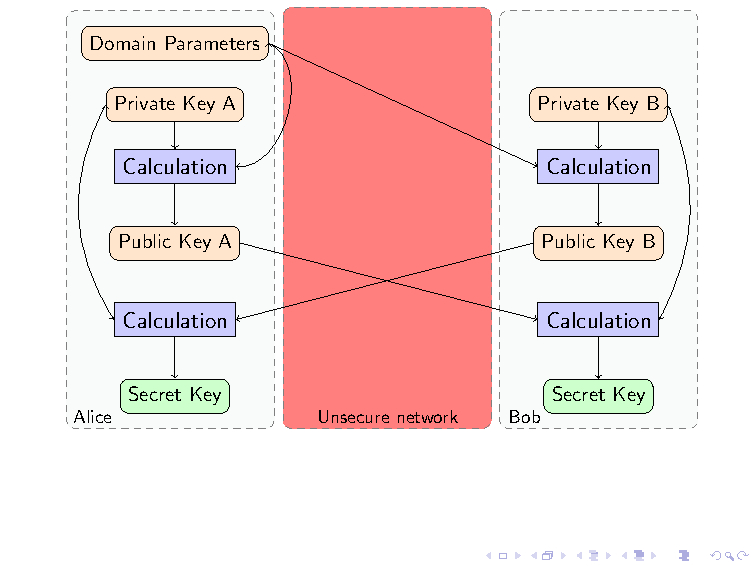
\includegraphics[trim=0.5cm 4cm 14cm 0cm,
height=5cm]{figures/diffie_hellman.pdf}

\end{frame}

%%%%%%%%%%%%%%%%%%%%%%%%%%%
% FRAME FOR CONFIGURATONS %
%%%%%%%%%%%%%%%%%%%%%%%%%%%

\begin{frame}

\begin{itemize}
  \item Domain parameters created by one person (Alice)
  \item Private key created by each one and not sended
  \item Public key computed with the domain parameters and the private key
  \item Secret key compute with the own private key and the public key of the
  other person
  \item Same secret key in each side
\end{itemize}  

\vspace{0.25cm}

\begin{itemize}
  \item Start with asymmetric keys
  \item Finish with symmetric key
\end{itemize}



\end{frame}
